
%-----------------------------------------------------------------------------------
%	PACKAGES AND OTHER DOCUMENT CONFIGURATIONS
%----------------------------------------------------------------------------------



\documentclass[11pt]{article}

\usepackage[top=2cm, bottom=3cm, left=2cm, right=2cm]{geometry}

\setlength{\parskip}{1em}
\setlength{\parindent}{4em}
\linespread{1.25}
\usepackage{apacite}
\setlength{\parindent}{0in}

\newcommand{\Var}{\mathrm{Var}}

\newcommand{\Cov}{\mathrm{Cov}}

\newcommand{\plim}{\rightarrow_{p}}

\usepackage{amsmath, amsfonts}
\usepackage{graphicx}
\usepackage{pdfpages}
\usepackage{bm}
\usepackage{listings}

% Expectation symbol
\newcommand{\E}{\mathrm{E}}
\newcommand{\V}{\mathrm{V}}

%----------------------------------------------------------------------------------
%	TITLE AND AUTHOR(S)
%----------------------------------------------------------------------------------

\title{PubPol 713 Assignment 3} % The article title


\author{Nathan Mather} % The article author(s) 

\date{\today} % An optional date to appear under the author(s)


%----------------------------------------------------------------------------------
\begin{document}
	
%------------------------------------------------------------------------------
%	TABLE OF CONTENTS & LISTS OF FIGURES AND TABLES
%------------------------------------------------------------------------------
\maketitle % Print the title/author/date block

\setcounter{tocdepth}{2} % Set the depth of the table of contents to show sections and subsections only

%\tableofcontents % Print the table of contents

%-------------------------------------------------------------
% Question 1 
%-------------------------------------------------------------
\section{ Question 1}

The results are displaying in the table below. The treatment effect is statistically significant. 

\begin{center}

	{
\def\sym#1{\ifmmode^{#1}\else\(^{#1}\)\fi}
\begin{tabular}{l*{1}{c}}
\hline\hline
                    &\multicolumn{1}{c}{esum18i}\\
\hline
Treatment indicator &       562.4\sym{**} \\
                    &     (183.6)         \\
[1em]
Constant            &      9274.3\sym{***}\\
                    &     (139.7)         \\
\hline
Observations        &       10812         \\
\hline\hline
\multicolumn{2}{l}{\footnotesize Standard errors in parentheses}\\
\multicolumn{2}{l}{\footnotesize \sym{*} \(p<0.05\), \sym{**} \(p<0.01\), \sym{***} \(p<0.001\)}\\
\end{tabular}
}

	
\end{center}



%-------------------------------------------------------------
% Question 2
%-------------------------------------------------------------
\section{ Question 2}

First, I test the hypothesis of equal means for the treated and control group separately for each variable. 

\begin{center}
	\scalebox{0.80}{	
		{
\def\sym#1{\ifmmode^{#1}\else\(^{#1}\)\fi}
\begin{tabular}{l*{10}{c}}
\hline\hline
                    &\multicolumn{1}{c}{sex}&\multicolumn{1}{c}{race}&\multicolumn{1}{c}{age}&\multicolumn{1}{c}{totch18}&\multicolumn{1}{c}{child\_miss}&\multicolumn{1}{c}{bfeduca}&\multicolumn{1}{c}{ed\_miss}&\multicolumn{1}{c}{bfyrearn}&\multicolumn{1}{c}{earn\_miss}&\multicolumn{1}{c}{est10}\\
\hline
Treatment indicator &     -0.0114         &     0.00853         &      -0.226         &    0.000434         &    0.000703         &       0.125\sym{**} &    -0.00767\sym{***}&      -39.51         &     0.00185         &     -0.0282         \\
                    &   (0.00965)         &    (0.0159)         &     (0.206)         &    (0.0273)         &   (0.00556)         &    (0.0433)         &   (0.00231)         &     (72.07)         &   (0.00741)         &    (0.0955)         \\
\hline
Observations        &       10812         &       10812         &       10812         &       10812         &       10812         &       10812         &       10812         &       10812         &       10812         &       10812         \\
\hline\hline
\multicolumn{11}{l}{\footnotesize Standard errors in parentheses}\\
\multicolumn{11}{l}{\footnotesize \sym{*} \(p<0.05\), \sym{**} \(p<0.01\), \sym{***} \(p<0.001\)}\\
\end{tabular}
}

	}
\end{center}

Most of the variables are not statistically different with the exception of years of schooling at baseline and missing education. Even just two significant results are suggestive of a significant ex ante difference in treatment and control groups. This could indicate a problem with randomization if it was not carried out properly in the field. Even if randomization was successful, however, we may have by chance ended up with uneven characteristics. In this case, it will still be a good idea to account for these known ex post differences. \par 

to check this in another way I run the following regression 

$$ treat_i = \bf{B}\bf{X_i} $$

where $\bf{X_i}$ is a vector of the observed characteristics from above. I then run an F test on the joint significance of all these variables to determine joint orthogonality between the treatment and control. The F test is  1.76 which translates into Prob $> F  =  0.0697$. This test simply reinforces the findings from the individual t-tests. 



%-------------------------------------------------------------
% Question 3
%-------------------------------------------------------------
\section{ Question 3}

The results from running the model described are below. 

\begin{center}
	
		{
\def\sym#1{\ifmmode^{#1}\else\(^{#1}\)\fi}
\begin{tabular}{l*{1}{c}}
\hline\hline
                    &\multicolumn{1}{c}{(1)}\\
                    &\multicolumn{1}{c}{earnings 18 months after}\\
\hline
Treatment indicator &       599.7\sym{***}\\
                    &     (169.0)         \\
[1em]
sex                 &      4192.6\sym{***}\\
                    &     (174.0)         \\
[1em]
race                &      -627.5\sym{***}\\
                    &     (103.8)         \\
[1em]
age                 &      -19.76\sym{*}  \\
                    &     (8.175)         \\
[1em]
totch18             &       234.5\sym{***}\\
                    &     (63.52)         \\
[1em]
child\_miss          &       747.1\sym{*}  \\
                    &     (307.9)         \\
[1em]
bfeduca             &       737.3\sym{***}\\
                    &     (48.32)         \\
[1em]
ed\_miss             &      8000.5\sym{***}\\
                    &     (902.5)         \\
[1em]
bfyrearn            &       0.634\sym{***}\\
                    &    (0.0244)         \\
[1em]
earn\_miss           &      1257.8\sym{***}\\
                    &     (230.2)         \\
[1em]
site\_num            &      -85.01\sym{***}\\
                    &     (17.28)         \\
[1em]
Constant            &      -694.5         \\
                    &     (631.8)         \\
\hline
Observations        &       10812         \\
\hline\hline
\multicolumn{2}{l}{\footnotesize Standard errors in parentheses}\\
\multicolumn{2}{l}{\footnotesize \sym{*} \(p<0.05\), \sym{**} \(p<0.01\), \sym{***} \(p<0.001\)}\\
\end{tabular}
}

	
\end{center}

These are worth including because they are observable characteristics that are likely to impact outcomes. Even in what is ex anti totally random sampling, without stratification we may end up with uneven ex post observables across treatment and control. Including these in the model ensures that these uneven observables are accounted for. As we saw in question 2, there are significant differences of observables. Furthermore, even small differences in observables can significantly impact the estimate of the treatment effect if those observables have a strong impact on the outcome. \par 

The treatment effect is a bit higher in this model than in the treatment effect from question 1. This is a bit surprising since the treated group was more likely to have high Previous education (found in question 2), and high previous education is associated with higher earnings after treatment (as seen in the bfeduca coefficient above). If left unaccounted for, as in question 1, some of the impact of previous education would have been attributed to the treatment effect in question 1. While a bit unexpected this result is not shocking as other observables differ as well and could easily net out to a higher treatment effect from uneven previous education. For example the relationship with missing education is working in the opposite direction. 


%-------------------------------------------------------------
% Question 4
%-------------------------------------------------------------
\section{ Question 4}

Let U be the error in the regression equation, T be the treatment variable, and X our matrix of covariates. The requirement for consistency of all the estimates under OLS generally is $ \E(U|X, T)=0$. That is the error term in the regression needs to be zero conditional on our covariates. We are also assuming the structure of this data generating process is linear in our parameters. Since we are only interested in interpreting the coefficient on the treatment effect, lets call it T, we can actually relax that assumption a bit. We need 

$$ \E[TU|X] = 0$$

This ensures that treatment is uncorrelated with the error conditional on the X's. This relaxes the assumption because the error no longer has to be zero conditional on X it just has to be uncorrelated with T. So we could, for example, have an omitted variable that impacts Y as long as it is uncorrelated with treatment T. 
\par


This is convincingly satisfied by the randomization of treatment and control. Error is zero conditional on treatment without any variables since as the sample tends to infinity covariates X should tend to be equally distributed to treatment and control. However, the idea here is that controlling for them anyway will improve the finite sample estimates.

%-------------------------------------------------------------
% Question 5
%-------------------------------------------------------------
\section{ Question 5}

The results of my propensity score regression are below
\begin{center}
	
	{
\def\sym#1{\ifmmode^{#1}\else\(^{#1}\)\fi}
\begin{tabular}{l*{1}{c}}
\hline\hline
                    &\multicolumn{1}{c}{(1)}\\
                    &\multicolumn{1}{c}{earnings 18 months after}\\
\hline
Treatment indicator &                     \\
sex                 &     -0.0270         \\
                    &    (0.0253)         \\
[1em]
race                &     0.00660         \\
                    &    (0.0152)         \\
[1em]
age                 &    -0.00119         \\
                    &   (0.00119)         \\
[1em]
totch18             &    0.000646         \\
                    &   (0.00924)         \\
[1em]
child\_miss          &      0.0308         \\
                    &    (0.0449)         \\
[1em]
bfeduca             &     0.00927         \\
                    &   (0.00704)         \\
[1em]
ed\_miss             &      -0.238         \\
                    &     (0.131)         \\
[1em]
bfyrearn            & -0.00000104         \\
                    &(0.00000355)         \\
[1em]
earn\_miss           &      0.0140         \\
                    &    (0.0336)         \\
[1em]
site\_num            &   -0.000415         \\
                    &   (0.00252)         \\
[1em]
Constant            &       0.134         \\
                    &    (0.0912)         \\
\hline
Observations        &       10812         \\
\hline\hline
\multicolumn{2}{l}{\footnotesize Standard errors in parentheses}\\
\multicolumn{2}{l}{\footnotesize \sym{*} \(p<0.05\), \sym{**} \(p<0.01\), \sym{***} \(p<0.001\)}\\
\end{tabular}
}

	
\end{center}


%-------------------------------------------------------------
% Question 6
%-------------------------------------------------------------
\section{ Question 6}


	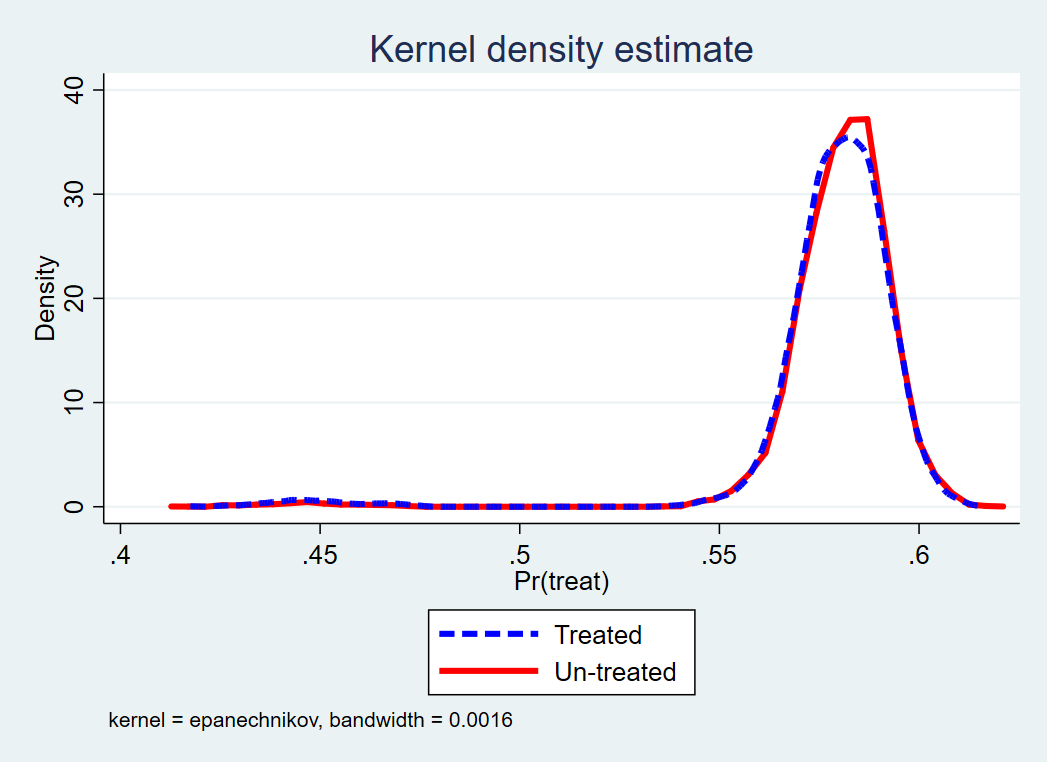
\includegraphics[width=1\linewidth]{6_kdens.png}

The densities do not appear to differ dramatically. This makes sense as it is based on a randomized trial. However there is some discrepancy around the peak which is consistent with the mild differences we observed above. In terms of the range of values in the density, the support of the treatment and control group don't exactly match but are extremely close (I would never expect them to match exactly). They are close enough that no observations will be excluded for lack of common support in the propensity score matching estimate. 


%-------------------------------------------------------------
% Question 7
%-------------------------------------------------------------
\section{ Question 7}

I did both a propensity score matching model with the "Nearest Neighbor matching" and, as a comparison, I ran an exact nearest neighbor matching model treating bfyrearn age bfeduca totch18 as continuous and adjusting for bias introduced by multiple continuous variables. 

\begin{center}
	
	{
\def\sym#1{\ifmmode^{#1}\else\(^{#1}\)\fi}
\begin{tabular}{l*{2}{c}}
\hline\hline
                    &\multicolumn{1}{c}{Propensity score matching}&\multicolumn{1}{c}{Nearest Neighbor match}\\
\hline
ATET                &                     &                     \\
r1vs0.Treatment indicator&       469.8\sym{*}  &       414.9         \\
                    &     (231.8)         &     (221.0)         \\
\hline
Observations        &       10812         &        9764         \\
\hline\hline
\multicolumn{3}{l}{\footnotesize Standard errors in parentheses}\\
\multicolumn{3}{l}{\footnotesize \sym{*} \(p<0.05\), \sym{**} \(p<0.01\), \sym{***} \(p<0.001\)}\\
\end{tabular}
}

	
\end{center}

The results of the propensity score matching are smaller than what we found in question 1. This is different than the OLS results in question 3. This result controls for ex post differences in observables between the treatment and the control. This differs from the OLS estimate in that it does not assume linearity in the parameters for the estimate of the ATET. That being said the propensity score assumes a functional form for the impact of observables on the probability of treatment and so it is still parametric.  



%-------------------------------------------------------------
% Question 8
%-------------------------------------------------------------
\section{ Question 8}

The simulated confounders gave an ATT estimate of 470.923 with a standard error of 241.364.

a) we are assuming that selection is a function of observables and this simulated confounder only. In other words that this satisfies the conditional independence assumption once we include this binary confounder. Let C be the confounder, then 
$ \E[y_{ji} | X, T, C] = \E[Y_{ij}|X,C] for j = 0,1$

b) The simulated confounder gave an ATT estimate of 692.847  with a standard error of 283.202. This is nt too far off from the original estimate which suggests that if there is a confounder of roughly equal importance to sex, which I used for the simulated probabilities,  our analysis is still in the right ball park. I think Ideally I would run this simulation for a grid of probabilities and determine at what point our conclusion from the estimates would drastically differ. Then, I can compare the distribution of this hypothetical confounder to any omitted variables the may be biasing the result. 


c) The strength is that it helps us think about the magnitude of how violations to our untestable assumptions would impact our estimates. The limitation is that it can't tell us anything about the probability of any of these confounding variables actually existing. For that, we need to use the variables we have as a reference and theory for what we think impacts our outcome. 


%-------------------------------------------------------------
% Appendix 
%-------------------------------------------------------------
\section{Appendix}
\subsection{Stata Code}
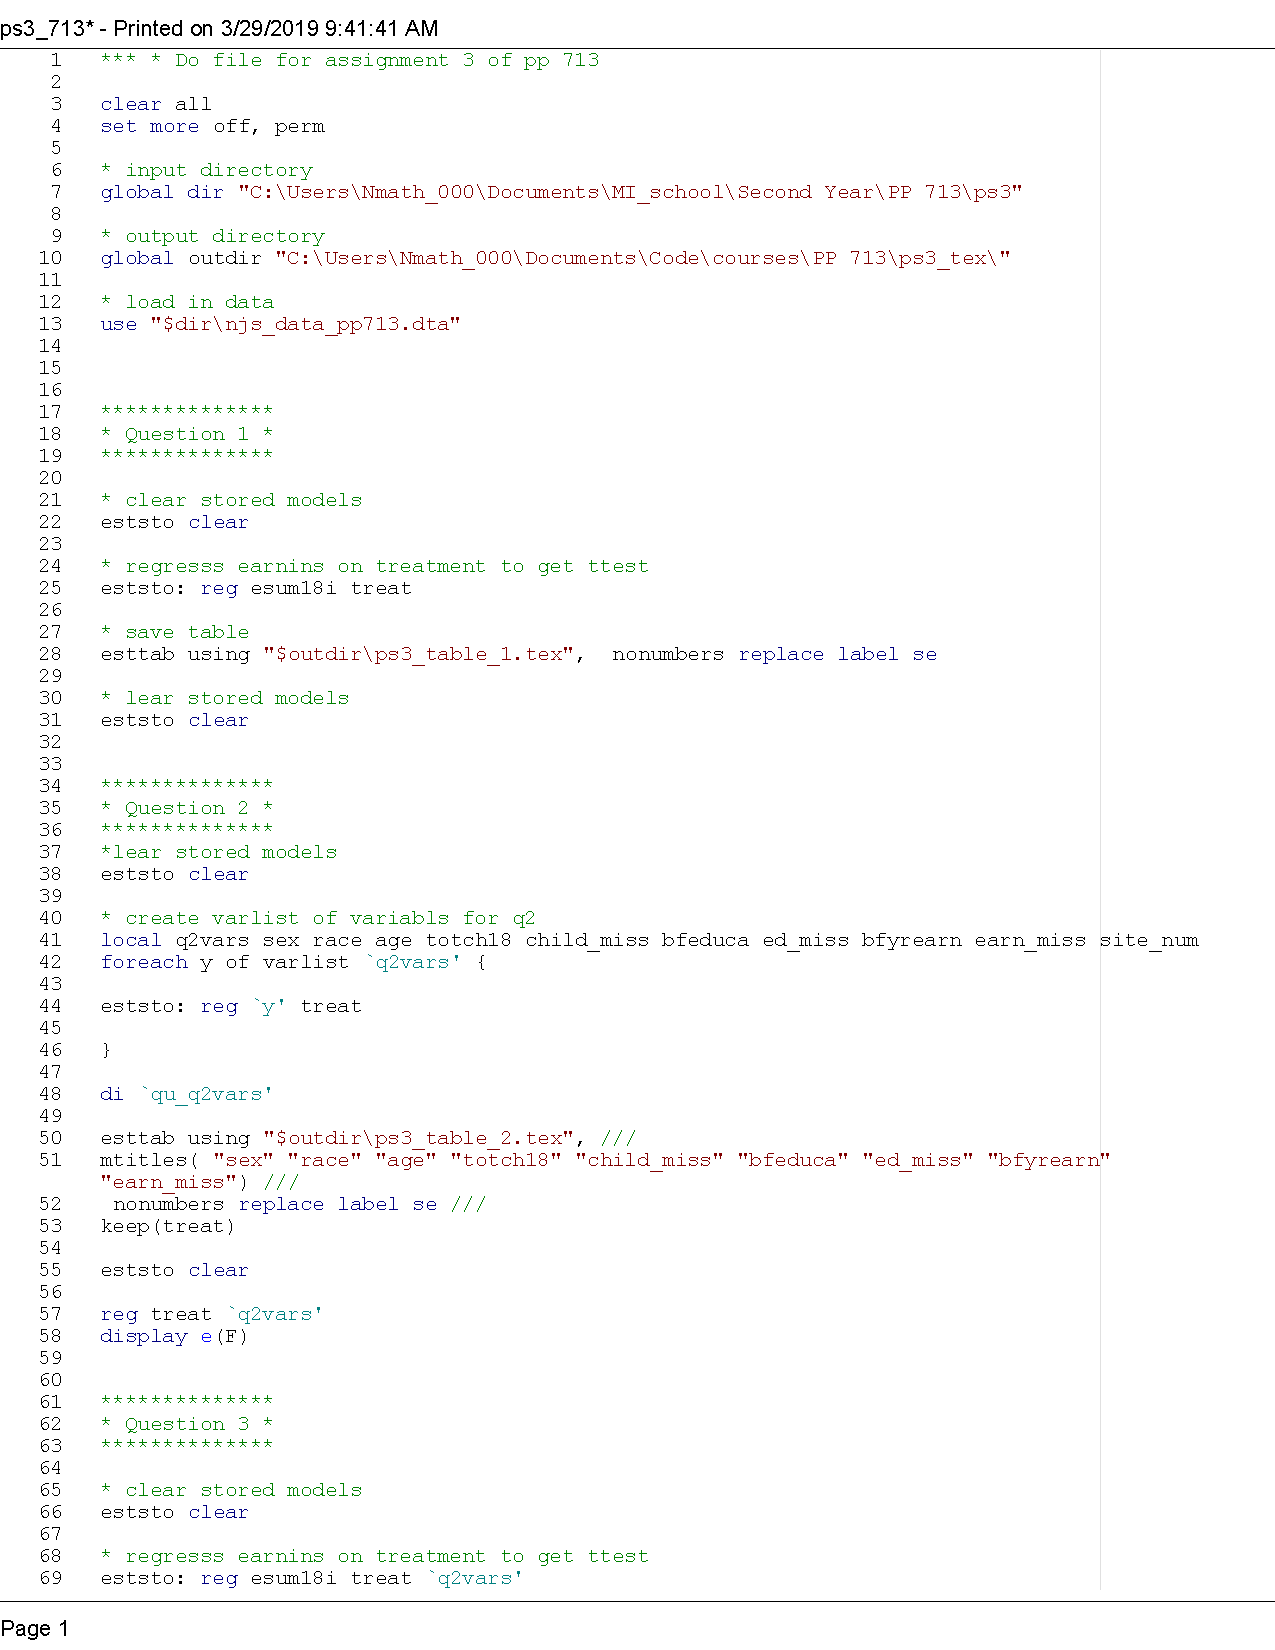
\includepdf[page=-]{pp713_ps3_stata_code.pdf}




%-----------------------------------------------
% end doc
%------------------------------------------------
\end{document}

